\documentclass[shrink, compress, mathserif, 10pt, xcolor=dvipsnames,
               aspectratio=169]{beamer}
\usetheme{Scale}

\usepackage{textcomp}
%%\usepackage[french]{babel}
\usepackage[T1]{fontenc}
\usepackage[utf8]{inputenc}
\usepackage{helvet}

\title{The NSIMD library}
\subtitle{Application to EFISPEC3D, the ground motion simulation}
\date{\today}
\author{Agenium Scale}

\begin{document}

\begin{frame}[plain]
  \maketitle
\end{frame}

\input{NSIMD-en.tex}

\begin{frame}{Application to EFISPEC3D}
  \begin{itemize}
    \item Ground motion simulation based on the Spectral Finite Element Method.
    \vspace{1em}
    \item Similar to SPECFEM3D, extracted from EFISPEC3D developed at BRGM
          (French geological survey).
    \vspace{1em}
    \item Unstructured mesh: elements share points at boundaries with neighbors
          $\longrightarrow$ indirection array to avoid storing points multiple
          times.
    \vspace{1em}
    \item Original code in written in Fortran.
    \vspace{1em}
    \item No/poor automatic vectorization (even with pragmas) on all
          architectures/compilers.
    \vspace{1em}
    \item Vectorization has to be done by using NSIMD.
  \end{itemize}
\end{frame}

\begin{frame}{Running times}
  \begin{center}
    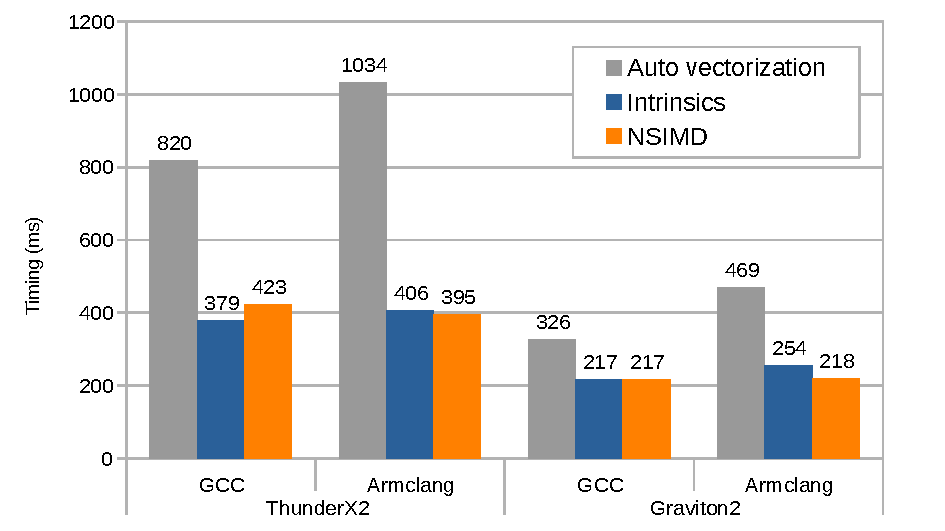
\includegraphics[width=0.55\textwidth]{timings.pdf}
  \end{center}
\end{frame}

\begin{frame}{Conclusion and links}
  \begin{itemize}
    \item
      One source code for all SIMD extensions.
    \item
      NSIMD has no overhead for scientific and industrial codes that do
      heavy computations.
    \item
      Increase in lisibility and maintainability of the code.
  \end{itemize}

  \vspace{2em}
  \begin{enumerate}
    \item EFISPEC3D: \url{https://www.brgm.fr/projet/efispec3d-prediction-numerique-sismogrammes-risque-sismique}
    \item NSIMD: \url{https://github.com/agenium-scale/nsimd}
    \item EFISPEC3D with NSIMD: \url{https://github.com/agenium-scale/EFISPEC3D}
    \item AGENIUM SCALE: \url{https://www.agenium-scale.com}
  \end{enumerate}
\end{frame}

\end{document}
